\chapter{Architektur}
%Graph mit allen Tools, Architektur in Graph zeigen
%Beschreibung alles Frameworks, die in Prototyp verwendet werden
%DI in Backend und DI in Frontend, reference auf Kapitel Theorie->DI

Die webbasierte Foto-Verwaltungs-Service wurde auf Basis des \textbf{MVC-}Pattern \textbf{(Kap. \ref{mvc})}. entwickelt, die aus drei Komponenten (Model, View und Controller) \textbf{(Abb. \ref{img:architectureMyApp})} besteht. Backend enthält das Model. Im Frontend-Teil der Web-Applikation befinden sich zwei weitere Komponente, View und Controller. View übernimmt die Verantwortung für die Gestaltung der Webseite und Controller wird in JavaScript implementiert, der die Client-Anfragen entsprechend bearbeitet.

Des Weiteren ist eine Datenbank für die Speicherung der Daten nötig. Die Web-Applikation ist nach dem \textit{Dependency Injection} konzipiert. Dies erlaubt einen freien Auswahl für die Verwendung der Datenbank. Falls eine SQL oder eine aus der NoSQL-Welt gewünscht wird, muss man nur die entsprechende Komponente ersetzen.

Der Zugriff auf Funktionen auf der Serverseite erfolgt über eine REST Server. Durch die Verwendung von REST API erfolgen die Client-Anfragen auf Basis des HTTP-Protokolls. Der Client (=Browser Anwendung) sendet HTTP-Request und erwartet HTTP-Response, in dem Fall des implementierten Prototyps im JSON-Format.

\begin{figure}[H]
\centering
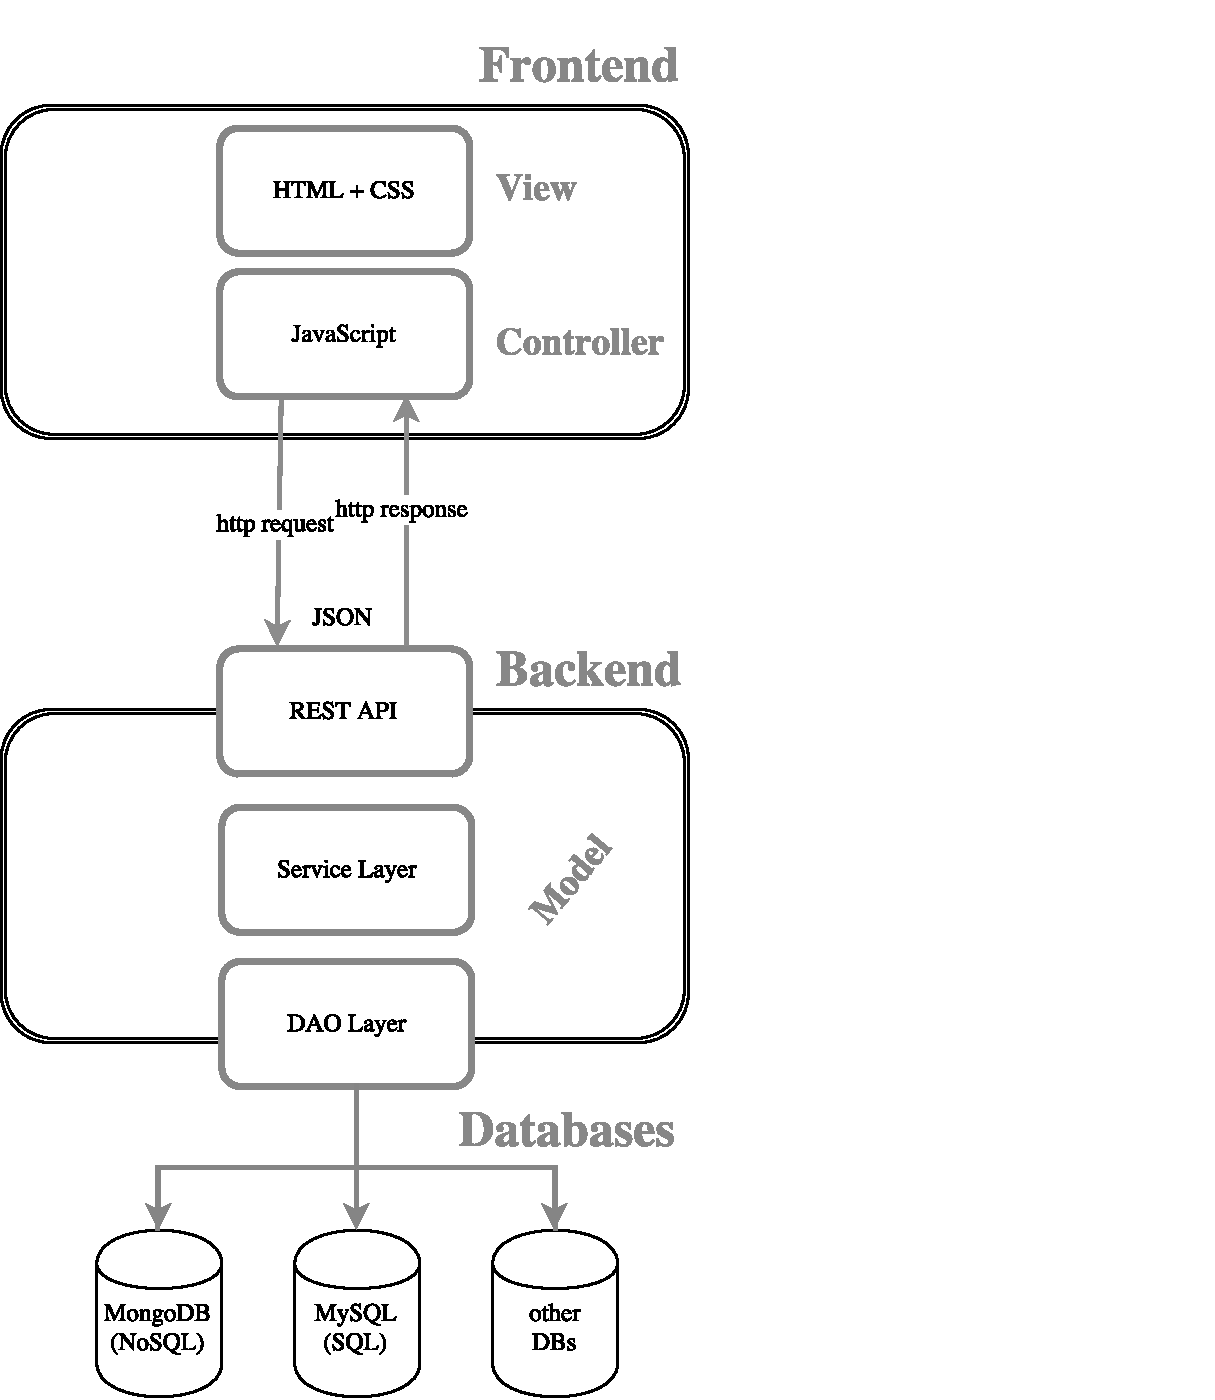
\includegraphics[trim = 0mm 0mm 0mm 0mm, clip, width=0.4\textwidth]{resources/architectureMyAppWithoutFrameworks}
\caption[Architektur-Prototyp]{Architektur-Prototyp}
\label{img:architectureMyApp}
\end{figure}

%\begin{wrapfigure}{r}{0.4\textwidth}
%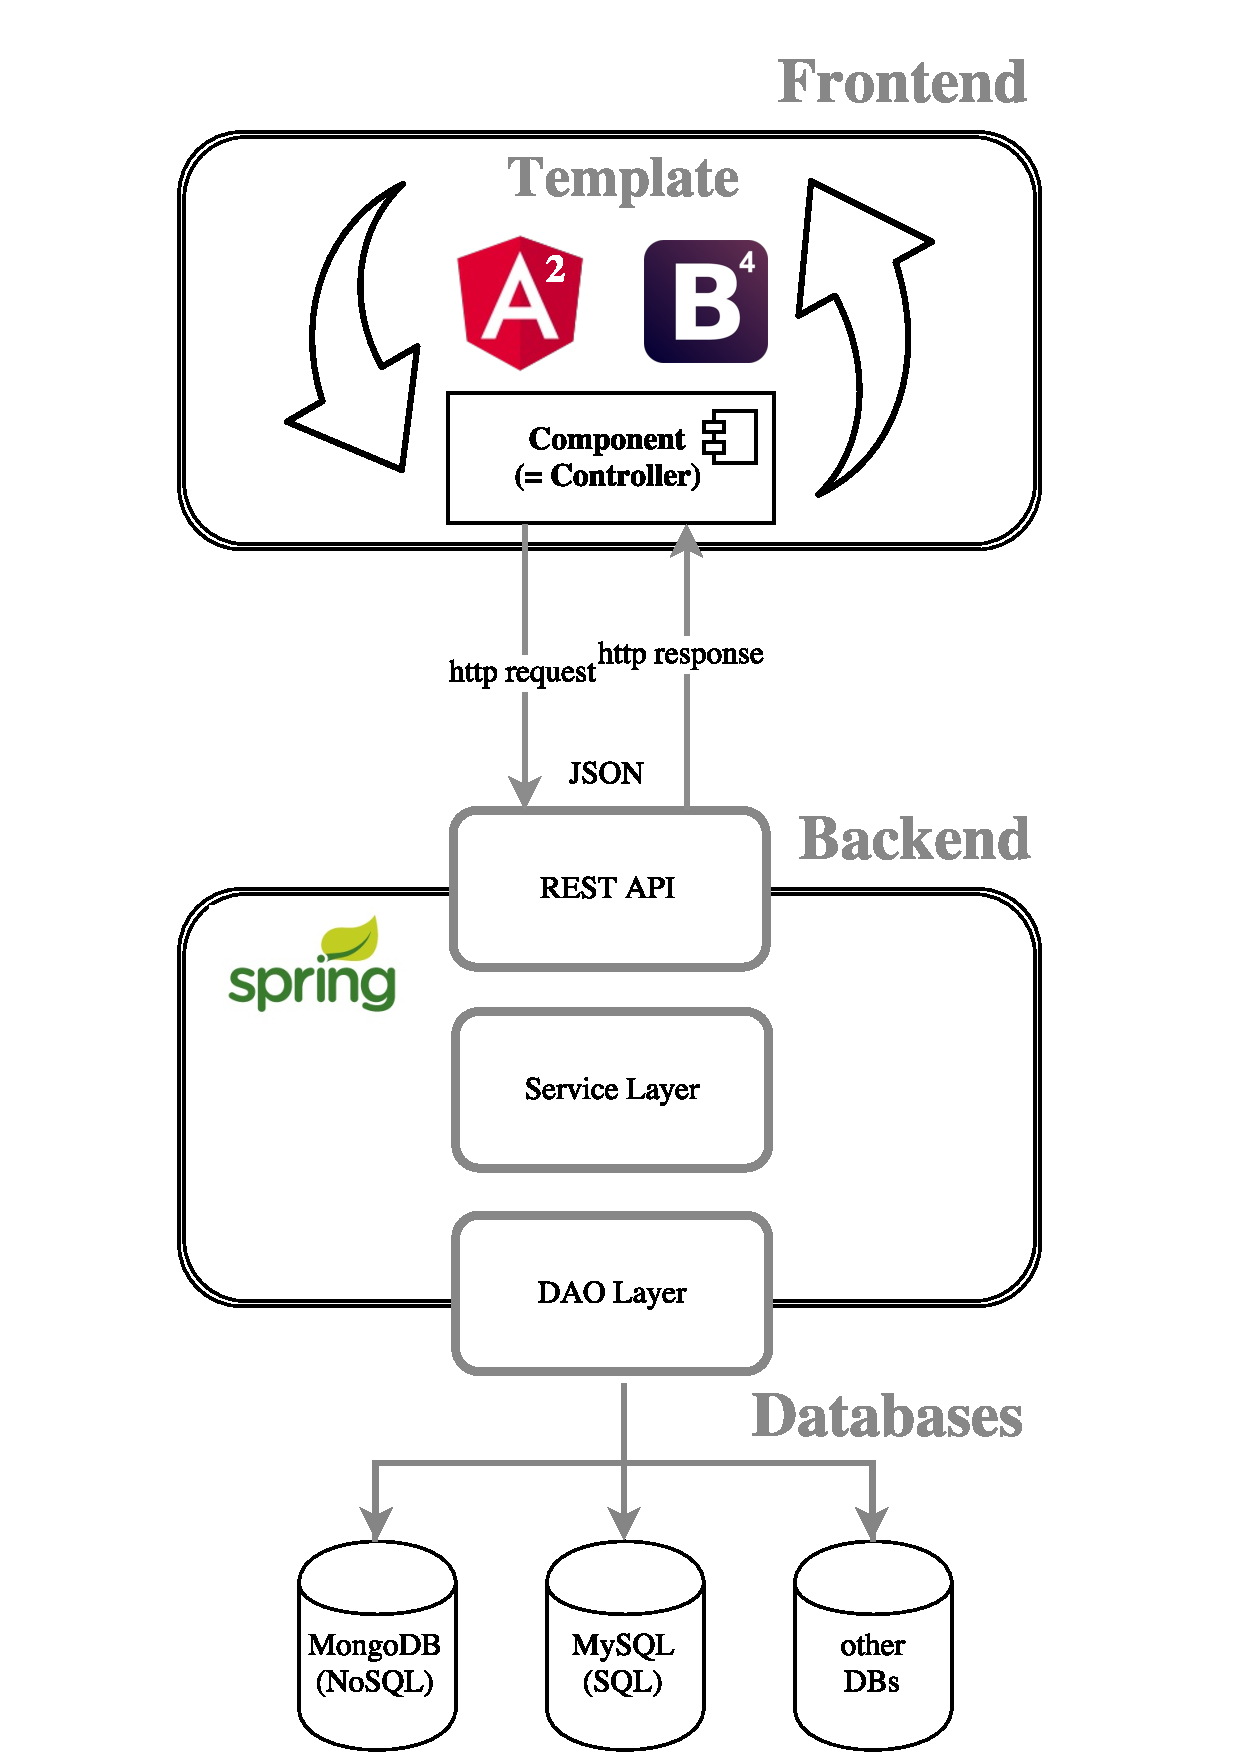
\includegraphics[trim = 20mm 0mm 30mm 9mm, clip, width=0.4\textwidth]{resources/architectureMyApp}
%\caption[Architektur-Prototyp]{\label{img:myArchitecture}Architektur-Prototyp}
%\end{wrapfigure}

\section{Präsentationsschicht (Frontend)}
AngularJS 2

\section{Logikschicht (Backend)}
\subsection{Rest Server}

\subsection{Spring MVC}
\section{Datenhaltungsschicht (Databases)}
Im Vergleich zu den relationalen Datenbanken, die sich als eine strukturierte Sammlung von Tabellen (den Relationen) vorstellen, in welchen Datensätze abgespeichert sind, eignen sich NoSQL-Datenbanken zur unstrukturierter Daten, die einen nicht-relationalen Ansatz verfolgen. 

\subsection{NoSQL-Datenbanken}
Der Begriff NoSQL steht nicht für 'kein SQL', sondern für 'nicht nur SQL' (Not only SQL). Das Ziel von NoSQL ist, relationale Datenbanken sinnvoll zu ergänzen, wo sie Defizite aufzeigen. Entstanden ist dieses Konzept in erster Linie als Antwort zur Unflexibilität, sowie zur relativ schwierigen Skalierbarkeit von klassischen Datenbanksystemen, bei denen die Daten nach einem stark strukturierten Modell gespeichert werden müssen.\footnote{MySQL vs. MongoDB: \url{http://www.computerwoche.de/a/datenbanksysteme-fuer-web-anwendungen-im-vergleich,2496589}, zugegriffen am 3. Januar 2016} Dokumentdatenbanken gruppieren die Daten in einem strukturierten Dokument, typischerweise in einer JSON-Datenstruktur. Auch \mongo, siehe dazu Abschnitt \ref{mongo} verfolgt diesen Ansatz und bietet darauf aufbauend eine reichhaltige Abfragesprache und Indexe auf einzelne Datenfelder. Die Möglichkeiten der Replikation und des Shardings zur stufenlosen und unkomplizierten Skalierung der Daten und Zugriffe macht \mongo\ auch für stark frequentierte Websites äußerst interessant.(\cite{Hollosi.2012}, Kapitel 14, Seite 435)

Beispiele für NoSQL-Datenbanken....:
\begin{multicols}{2}
\begin{itemize}
\item CouchDB
\item MongoDB
\item Redis
\item Google BigTable
\item Amazon Dynamo
\item Apache Cassandra
\item Hbase (ApacheHadoop)
\item Twitter Gizzard
\item weitere…
\end{itemize}
\end{multicols}
Jede NoSQL-Datenbanke verfolgt seine Ziele und welche sie genau verfolgen, beschreibt der Abschnitt \ref{categoryNoSQL}, in dem verschiedene Kategorien von NoSQL-Datenbanken vorgestellt werden.

\subsubsection{Kategorien von NoSQL-Systemen}\label{categoryNoSQL}

\paragraph{Key-Value-Datenbanken}

Eine Key-Value-Datenbank \textit{(Key-Value Store)} ist eine Datenbank, in der die Daten in Form von Schlüssel-Werte-Paaren abgespeichert werden. Der Schlüssel verweist dabei auf einen eindeutigen (meist in Binär- oder Zeichenketten-Format vorliegenden) Wert\footnote{NoSQL: Key-Value-Datenbank Redis im Überblick: \url{https://www.heise.de/developer/artikel/NoSQL-Key-Value-Datenbank-Redis-im-Ueberblick-1233843.html}, zugegriffen am 17. Januar 2017}. Value kann oft beliebiger Datentyp wie Arrays, Dokumente, Objekte, Bytes etc. sein. Siehe dazu die Abbildung \ref{img:kvdb} mit einem Beispiel:


\paragraph{Spaltenorientierte Datenbanken}

In einer spaltenorientierten Datenbank \textit{(Column Store)}, wie der Name vermuten lässt, werden die Datensätze spalten- statt zeilenweise abgespeichert. Durch die spaltenorientierte Abspeicherung der Daten wird der Lesezugriff stark beschleunigt, da keine unnötigen Informationen mehr gelesen werden, stattdessen nur diejenigen, die wirklich benötigt wurden. Dadurch wird der Schreibprozess aber erschwert, falls die schreibenden Daten aus mehreren Spalten bestehen werden, auf die entsprechend zugegriffen werden muss. Der Schreibprozess wird sich in diesem Fall etwas verlangsamen.


\paragraph{Graphen-Datenbanken}
Eine Graphen-Datenbank \textit{(Graph database)} ist weitere Kategorie aus der NoSQL Gruppe, in der die Daten anhand eines Graphen dargestellt und abgespeichert werden.


Wie der Abbildung \ref{img:gdb} zu entnehmen ist, bestehen Graphen grundsätzlich aus Knoten \textit{(Node)} und Kanten \textit{(Edge)}. Dabei stellen die Kanten die Verbindungen zwischen den einzelnen Knoten dar.

\paragraph{Dokumentenorientierte Datenbanken}

Eine Datenbank, in der die Daten in Form von Dokumenten abgespeichert werden, ist als eine dokumentenorientierte Datenbank \textit{(Document Store)} zu definieren. In diesem Zusammenhang ist ein Dokument als eine Zusammenstellung bestimmter Daten zu verstehen, das mit einem eindeutigen Identifikator angesprochen werden kann. Da die Daten in der dokumentenorientierte Datenbank nicht in Form von Tabellen, sondern in Form von Dokumenten abgespeichert werden, ergibt sich daraus keinen Strukturzwang. Als Beispiel ist aus der Abbildung \ref{img:dodb} zwei Dokumente im \textbf{JSON}-Format zu entnehmen, die sich voneinander gänzlich unterscheiden.


Möchte man ein bestimmtes Dokument erweitern, so kann man es einfach tun, da eine dokumentenorientierte Datenbank strukturfrei ist. Weitere Datenformate sind beispielsweise YAML\footnote{YAML: \url{http://www.yaml.org/start.html}} (angelehnt an XML) oder XML\footnote{XML: \url{https://www.xml.com/}} selbst.










\section{Frameworks}





Alllgemeine Architektur
    Überblick
    Datenschicht
        Nosql

Frameworks